% !TEX root = ../main_zh.tex
\chapter{IS--LM 模型}
\label{ch:islm}

第~\ref{ch:keynes}~章的凯恩斯交叉，是在\emph{给定}利率的前提下确定产出的：它告诉我们计划支出与 $45^\circ$ 线在何处相交，却把利率 $r$ 当作外界递进来的一个数字。然而 $r$ 本身就是一个均衡价格——它是流动性的价格——并且会随产出的变化而变化。IS--LM 模型把这个回路闭合起来。它仍然假定价格水平固定（我们依旧处在短期），转而去寻找使两个市场\emph{同时}出清的 $(Y,r)$ 组合：一个是商品市场，由 \emph{IS} 曲线刻画；另一个是货币市场，由 \emph{LM} 曲线刻画。我们将会看到，财政政策作用于前一条曲线，货币政策作用于后一条曲线，而两者的相互作用，正是使上一章那个简单乘数被高估的原因。

\section{IS 曲线}

IS 曲线是使商品市场处于均衡——即计划支出等于产出——的全部 $(Y,r)$ 组合的集合。曲线上的每一点，都对应着某个特定利率下的凯恩斯交叉均衡点。要看清它的形状，回忆一下：利率上升时投资下降，即 $I=I(r)$ 且 $I'(r)<0$。把投资写成 $r$ 的函数，再去解凯恩斯交叉，可得
\[
Y^{*} = \frac{1}{1-\mathrm{MPC}}\,\big(C_0 - \mathrm{MPC}\cdot T + I(r) + G + \mathrm{NX}\big),
\]
于是利率下降会抬高投资，使计划支出线向上平移，并经由乘数放大，抬高均衡产出。因此，沿着商品市场的均衡轨迹，产出与利率朝相反方向移动。

\begin{figure}[h]
\centering
\begin{tikzpicture}[scale=1.0]
  % ---- shared geometry: the two output levels live on one vertical grid ----
  \def\Yzero{2.8}   % Y0
  \def\Yone{5.6}    % Y1
  \def\xmax{7.4}

  % ================= TOP PANEL: Keynesian cross =================
  \begin{scope}[shift={(0,6.6)}]
    % axes
    \draw[-Latex] (0,0) -- (\xmax,0) node[right] {$Y$};
    \draw[-Latex] (0,0) -- (0,6.0) node[above] {$\mathrm{AD}$};
    % 45-degree line (reaches above the upper equilibrium Y1)
    \draw (0,0) -- (5.95,5.95);
    \node[above left=-2pt and -2pt] at (5.95,5.95) {$45^{\circ}$};
    % lower AE line (slope = MPC < 1): crosses 45-line at Y0
    \draw[line width=1.0pt] (0,1.4) -- (6.7,{1.4+0.5*6.7});
    % upper AE line: shifted up, crosses 45-line at Y1
    \draw[line width=1.0pt] (0,2.8) -- (6.0,{2.8+0.5*6.0});
    % equilibrium dots
    \fill (\Yzero,\Yzero) circle (1.5pt);
    \fill (\Yone,\Yone) circle (1.5pt);
    % upward-shift arrow
    \draw[-Latex] (0.85,1.9) to[bend left=32] (1.05,3.05);
    % vertical guides down to the Y axis
    \draw[densely dashed] (\Yzero,\Yzero) -- (\Yzero,0) node[below] {$Y_{0}$};
    \draw[densely dashed] (\Yone,\Yone)   -- (\Yone,0)   node[below] {$Y_{1}$};
  \end{scope}

  % ================= BOTTOM PANEL: the IS curve =================
  \begin{scope}[shift={(0,0)}]
    % axes
    \draw[-Latex] (0,0) -- (\xmax,0) node[right] {$Y$};
    \draw[-Latex] (0,0) -- (0,4.8) node[above] {$r$};
    % downward-sloping convex IS curve
    \def\rzero{3.0}  % r0 height (above Y0)
    \def\rone{1.3}   % r1 height (above Y1)
    \draw[line width=1.0pt,smooth,samples=120,domain=0.9:7.0]
      plot (\x,{4.6*exp(-0.42*\x)+0.45}) node[right] {$\mathrm{IS}$};
    % equilibrium points on the curve
    \fill (\Yzero,{4.6*exp(-0.42*\Yzero)+0.45}) circle (1.5pt);
    \fill (\Yone,{4.6*exp(-0.42*\Yone)+0.45}) circle (1.5pt);
    % vertical guides up to the top panel and down to the Y axis
    \draw[densely dashed] (\Yzero,4.8) -- (\Yzero,0) node[below] {$Y_{0}$};
    \draw[densely dashed] (\Yone,4.8)  -- (\Yone,0)  node[below] {$Y_{1}$};
    % horizontal guides marking r0 and r1
    \draw[densely dashed] (0,{4.6*exp(-0.42*\Yzero)+0.45}) -- (\Yzero,{4.6*exp(-0.42*\Yzero)+0.45});
    \draw[densely dashed] (0,{4.6*exp(-0.42*\Yone)+0.45})  -- (\Yone,{4.6*exp(-0.42*\Yone)+0.45});
    \node[left] at (0,{4.6*exp(-0.42*\Yzero)+0.45}) {$r_{0}$};
    \node[left] at (0,{4.6*exp(-0.42*\Yone)+0.45})  {$r_{1}$};
    % downward arrow on the r axis from r0 to r1
    \draw[-Latex] (-0.95,{4.6*exp(-0.42*\Yzero)+0.45}) to[bend right=30] (-0.95,{4.6*exp(-0.42*\Yone)+0.45+0.05});
  \end{scope}
\end{tikzpicture}

\caption{IS 曲线的推导。上图中，利率从 $r_0$ 降到 $r_1$ 使投资增加，把计划支出线向上推，凯恩斯交叉均衡从 $Y_0$ 移到 $Y_1$。把每一个利率与它所对应的产出画在一起（下图），就描出了向下倾斜的 IS 曲线。}
\label{fig:macro-15}
\end{figure}

\defn{IS 曲线}{
\emph{IS 曲线}是使计划支出等于产出（商品市场出清）的 $(Y,r)$ 组合的轨迹。由于利率越低则投资越高、从而均衡产出越高，IS 曲线\emph{向下}倾斜。
}

图~\ref{fig:macro-15} 把生成它的两幅图叠在一起。除利率以外，凡是会移动凯恩斯交叉均衡的因素——$G$ 的变动、税收的变动、自发消费或自发投资的变动、净出口的变动——都会使\emph{整条} IS 曲线移动；而利率本身的变动，则是沿着曲线\emph{移动}。

\section{LM 曲线}

LM 曲线来自货币市场。货币数量论 $MV = PY$ 可以读作一个关于货币需求的命题：为了在流通速度 $V$ 之下完成名义交易量 $PY$，公众希望持有
\[
M^{d} = \frac{PY}{V}.
\]
这里流通速度并非常数；它随利率上升而上升，即 $V=V(r)$、$V'(r)>0$，因为利率越高，持有不生息货币的机会成本越大，于是每一单位货币的周转次数增加，所需持有的货币就越少。与此相对，货币供给由央行设定，与利率无关：在图中它是一条垂直线。

\begin{figure}[h]
\centering
\begin{tikzpicture}[scale=1.0]
  % axes
  \draw[-Latex] (0,0) -- (7.6,0) node[right] {$M$};
  \draw[-Latex] (0,0) -- (0,5.8) node[above] {$r$};
  % vertical money-supply line M^s (perfectly inelastic), thick = primary
  \draw[line width=1.2pt] (4.3,0) -- (4.3,5.4) node[above] {$M^{s}$};
  % downward-sloping money-demand curve M^d : r = k/(M - a)
  % chosen so it crosses M^s at a sensible interior r
  \draw[semithick,domain=0.95:7.2,smooth,variable=\x,samples=160]
        plot ({\x},{1.55/(\x-0.55)+0.18}) node[right] {$M^{d}$};
  % equilibrium point: x=4.3 on the demand curve
  \pgfmathsetmacro{\req}{1.55/(4.3-0.55)+0.18}
  \fill (4.3,\req) circle (1.6pt);
  % dashed guide to the r axis
  \draw[densely dashed] (4.3,\req) -- (0,\req) node[left] {$r^{*}$};
\end{tikzpicture}

\caption{货币市场。货币供给 $M^{s}$ 是垂直的（由央行设定）；货币需求 $M^{d}$ 随利率向下倾斜。两者的交点确定了均衡利率。}
\label{fig:macro-16}
\end{figure}

图~\ref{fig:macro-16} 中的均衡，钉住了在给定产出与价格下使货币市场出清的那个利率。现在让产出上升。$Y$ 越高意味着交易越多，于是在每一个利率水平上货币需求都更大，需求曲线向右移动。供给既然固定，利率就必须上升，把货币需求压回到既有的货币存量上。

\begin{figure}[h]
\centering
\begin{tikzpicture}[scale=1.0]
  % axes
  \draw[-Latex] (0,0) -- (8.6,0) node[right] {$M$};
  \draw[-Latex] (0,0) -- (0,6.4) node[above] {$r$};
  % vertical money supply M^s fixed
  \def\Ms{4.6}
  \draw[line width=1.2pt] (\Ms,0) -- (\Ms,6.0);
  \node[above] at (\Ms,6.0) {$M^{s}$};
  % money demand curves: rectangular-hyperbola shape r = k/M
  % M^{d_1} : original demand, equilibrium r_1 at M = Ms
  \def\rone{1.7}
  \pgfmathsetmacro{\kone}{\rone*\Ms}      % so that k/Ms = r_1
  \draw[semithick,domain=1.55:8.1,smooth,variable=\x,samples=160]
        plot ({\x},{\kone/\x});
  \node[below right] at (8.1,{\kone/8.1}) {$M^{d_1}$};
  % M^{d_2} : higher demand after GDP rises (shifted right), equilibrium r_2 at M = Ms
  \def\rtwo{3.0}
  \pgfmathsetmacro{\ktwo}{\rtwo*\Ms}      % so that k/Ms = r_2
  \draw[semithick,domain=2.35:8.3,smooth,variable=\x,samples=160]
        plot ({\x},{\ktwo/\x});
  \node[right] at (8.3,{\ktwo/8.3}) {$M^{d_2}$};
  % equilibrium points
  \fill (\Ms,\rone) circle (1.6pt);
  \fill (\Ms,\rtwo) circle (1.6pt);
  % dashed guides to the r-axis
  \draw[densely dashed] (\Ms,\rone) -- (0,\rone) node[left] {$r_1$};
  \draw[densely dashed] (\Ms,\rtwo) -- (0,\rtwo) node[left] {$r_2$};
  % upward arrow on the r-axis showing r rises
  \draw[-Latex] (-0.62,\rone) -- (-0.62,\rtwo);
  % single arrow showing the rightward shift of demand (in blank space)
  \draw[-Latex] (5.0,1.55) -- (5.95,2.2);
\end{tikzpicture}

\caption{产出上升使货币需求曲线向右移动；货币供给固定，均衡利率随之从 $r_0$ 上升到 $r_1$。}
\label{fig:macro-17}
\end{figure}

把这些 $(Y,r)$ 组合收集起来——产出越高，越需要更高的利率来维持货币市场的平衡——就描出了 LM 曲线。

\begin{figure}[h]
\centering
\begin{tikzpicture}[scale=1.0]
  % axes
  \draw[-Latex] (0,0) -- (0,5.4) node[above] {$r$};
  \draw[-Latex] (0,0) -- (7.6,0) node[right] {$Y$};
  % LM curve: upward-sloping convex locus, nearly flat at low Y, steep at high Y
  \draw[line width=1.2pt,smooth,samples=120,domain=0.5:6.2]
        plot (\x,{0.7+0.085*(\x-0.5)^2});
  \node[right] at (6.25,{0.7+0.085*(6.2-0.5)^2}) {$\mathrm{LM}$};
\end{tikzpicture}

\caption{LM 曲线：使货币市场出清的产出与利率组合的轨迹。它向上倾斜，因为产出越高则货币需求越大，从而使市场出清的利率越高。}
\label{fig:macro-18}
\end{figure}

\defn{LM 曲线}{
\emph{LM 曲线}（流动性偏好--货币供给，liquidity preference--money supply）是在给定实际货币供给下使货币市场出清的 $(Y,r)$ 组合的轨迹。由于产出越高则货币需求越大、从而均衡利率越高，LM 曲线\emph{向上}倾斜。
}

什么会使整条 LM 曲线移动？任何改变实际货币供给 $M/P$ 的因素。名义货币供给增加，意味着在任意产出水平上，市场都在更低的利率上出清，于是 LM 曲线向下（等价地，向右）移动。

\begin{figure}[h]
\centering
\begin{tikzpicture}[scale=1.0]
  %================ LEFT PANEL: money market ================
  \begin{scope}[shift={(0,0)}]
    % axes
    \draw[-Latex] (0,0) -- (6.4,0) node[right] {$M$};
    \draw[-Latex] (0,0) -- (0,5.6) node[above] {$r$};
    % money demand M^d : downward-sloping convex curve (rectangular hyperbola)
    \draw[semithick,smooth,samples=120,domain=0.62:5.9,variable=\x]
          plot ({\x},{2.7/(\x-0.25)+0.55}) ;
    \node[right] at (5.55,0.95) {$M^{d}$};
    % two vertical money-supply lines
    \def\Msa{3.3}\def\Msb{4.6}
    \draw[semithick] (\Msa,0) -- (\Msa,5.1) node[above] {$M^{s_{1}}$};
    \draw[semithick] (\Msb,0) -- (\Msb,5.1) node[above] {$M^{s_{2}}$};
    % equilibrium interest rates: r1 at inner supply, r2 (lower) at outer supply
    \pgfmathsetmacro{\rone}{2.7/(\Msa-0.25)+0.55}
    \pgfmathsetmacro{\rtwo}{2.7/(\Msb-0.25)+0.55}
    \fill (\Msa,\rone) circle (1.5pt);
    \fill (\Msb,\rtwo) circle (1.5pt);
    \draw[densely dashed] (0,\rone) -- (\Msa,\rone);
    \draw[densely dashed] (0,\rtwo) -- (\Msb,\rtwo);
    \node[left] at (0,\rone) {$r_{1}$};
    \node[left] at (0,\rtwo) {$r_{2}$};
  \end{scope}

  %================ connector ================
  \node at (7.6,2.7) {\Large $\Rightarrow$};

  %================ RIGHT PANEL: LM shift ================
  \begin{scope}[shift={(8.8,0)}]
    % axes
    \draw[-Latex] (0,0) -- (6.4,0) node[right] {$Y$};
    \draw[-Latex] (0,0) -- (0,5.6) node[above] {$r$};
    % upper (original) LM curve
    \draw[semithick,smooth,samples=120,domain=0.7:4.2,variable=\x]
          plot ({\x},{0.30*(\x-0.4)*(\x-0.4)+0.9});
    % lower/right (shifted) LM curve
    \draw[semithick,smooth,samples=120,domain=1.7:5.3,variable=\x]
          plot ({\x},{0.30*(\x-1.4)*(\x-1.4)+0.55});
    \node[above right] at (4.05,4.85) {$\mathrm{LM}$};
    % small shift arrows sitting in the blank gap between the two LM curves,
    % pointing down/right (direction of the shift) without touching either curve
    \draw[-Latex,semithick] (2.6,2.05) -- (2.95,1.6);
    \draw[-Latex,semithick] (3.4,3.0) -- (3.75,2.55);
  \end{scope}
\end{tikzpicture}

\caption{货币供给增加（从 $M^{s_1}$ 到 $M^{s_2}$）使每一产出水平下的市场出清利率下降，LM 曲线向下、向右移动。}
\label{fig:macro-19}
\end{figure}

价格水平上升的作用方向恰好相反。这里真正相关的量是\emph{实际}货币供给 $M/P$：$P$ 越高，$M/P$ 就越小，其效果与削减名义货币供给一模一样，使货币需求相对供给上升，把 LM 曲线向上推。

\begin{figure}[h]
\centering
\begin{tikzpicture}[scale=1.0]
  % ============================ LEFT PANEL: money market ============================
  \begin{scope}
    % axes
    \draw[-Latex] (0,0) -- (6.2,0) node[right] {$M$};
    \draw[-Latex] (0,0) -- (0,5.6) node[above] {$r$};
    % vertical money supply M^s
    \draw[line width=1.0pt] (3.9,0) -- (3.9,5.3);
    \node[above] at (3.9,5.3) {$M^{s}$};
    % money demand M^{d1} (lower/left convex curve): hyperbola passing through (3.9, r1)
    % r1 = 1.5 at M=3.9  => k1 = 1.5*3.9 = 5.85
    \draw[smooth,samples=120,domain=1.18:5.9,variable=\x] plot ({\x},{5.85/\x});
    \node[below right] at (5.9,5.85/5.9) {$M^{d1}$};
    % money demand M^{d2} (upper/right convex curve): hyperbola passing through (3.9, r2)
    % r2 = 2.85 at M=3.9  => k2 = 2.85*3.9 = 11.115
    \draw[smooth,samples=120,domain=2.05:5.9,variable=\x] plot ({\x},{11.115/\x});
    \node[below right] at (5.9,11.115/5.9) {$M^{d2}$};
    % equilibrium points on the M^s line
    \fill (3.9,1.5) circle (1.4pt);
    \fill (3.9,2.85) circle (1.4pt);
    % dashed horizontal guides to the r-axis
    \draw[densely dashed] (0,1.5) -- (3.9,1.5);
    \draw[densely dashed] (0,2.85) -- (3.9,2.85);
    \node[left] at (0,1.5) {$r_1$};
    \node[left] at (0,2.85) {$r_2$};
    % up-arrow on the r-axis between r1 and r2
    \draw[-Latex] (0.42,1.55) -- (0.42,2.80);
    % small arrows in the blank gap between M^{d1} and M^{d2}, indicating the rightward/upward shift
    \draw[-Latex] (2.0,3.55) -- (2.5,4.05);
    \draw[-Latex] (2.85,2.6) -- (3.35,2.95);
  \end{scope}

  % ============================ CONNECTOR ============================
  \node[scale=2.4] at (7.5,2.6) {$\Rightarrow$};

  % ============================ RIGHT PANEL: LM curve ============================
  \begin{scope}[xshift=9.0cm]
    % axes
    \draw[-Latex] (0,0) -- (6.2,0) node[right] {$Y$};
    \draw[-Latex] (0,0) -- (0,5.6) node[above] {$r$};
    % lower LM curve (convex, upward sloping): r = 0.55 + 0.10*(Y)^2 over a shifted range
    \draw[smooth,samples=120,domain=0.4:5.2,variable=\x]
        plot ({\x},{0.55+0.135*(\x)*(\x)});
    % upper LM curve: same shape shifted up by ~0.9
    \draw[smooth,samples=120,domain=0.4:4.85,variable=\x]
        plot ({\x},{1.45+0.135*(\x)*(\x)});
    \node[above left] at (4.85,1.45+0.135*4.85*4.85) {$\mathrm{LM}$};
    % small up-arrows in the blank gap between the two LM curves (clear of both)
    \draw[-Latex] (2.55,0.55+0.135*2.55*2.55+0.20) -- (2.55,1.45+0.135*2.55*2.55-0.14);
    \draw[-Latex] (3.65,0.55+0.135*3.65*3.65+0.20) -- (3.65,1.45+0.135*3.65*3.65-0.14);
  \end{scope}
\end{tikzpicture}

\caption{价格水平上升抬高名义货币需求（压低实际货币供给 $M/P$）；每一产出水平下的市场出清利率上升，LM 曲线向上移动。}
\label{fig:macro-20}
\end{figure}

\state{两条曲线怎么读}{
IS 曲线刻画商品市场，由\emph{财政}变量（$G$、$T$、自发支出）使其移动。LM 曲线刻画货币市场，由\emph{货币}变量——名义货币供给与价格水平——使其移动，二者都是通过实际货币供给 $M/P$ 起作用的。
}

\section{均衡}

把两条曲线画在同一张图上，横轴为产出，纵轴为利率，唯一的交点给出使\emph{两个}市场都出清的组合 $(Y_0,r_0)$。因果关系是双向传递的：利率通过投资帮助决定产出，产出又通过货币需求帮助决定利率。

\begin{figure}[h]
\centering
\begin{tikzpicture}[scale=1.0]
  % axes
  \draw[-Latex] (0,0) -- (8.2,0) node[right] {$Y$};
  \draw[-Latex] (0,0) -- (0,6.0) node[above] {$r$};
  % IS curve: downward sloping
  \draw[line width=1pt] (1.1,4.7) -- (6.6,1.0) node[below right] {$\mathrm{IS}$};
  % LM curve: upward sloping
  \draw[line width=1pt] (1.1,1.4) -- (7.0,5.1) node[above right] {$\mathrm{LM}$};
  % equilibrium intersection: solve the two lines
  % IS: from (1.1,4.7) to (6.6,1.0): slope = (1.0-4.7)/(6.6-1.1) = -0.6727, r = 4.7 -0.6727(Y-1.1)
  % LM: from (1.1,1.4) to (7.0,5.1): slope = (5.1-1.4)/(7.0-1.1) = 0.6271, r = 1.4 +0.6271(Y-1.1)
  % set equal: 4.7 -0.6727(Y-1.1) = 1.4 +0.6271(Y-1.1)
  % 3.3 = 1.2998(Y-1.1) -> Y-1.1 = 2.539 -> Y = 3.639, r = 1.4+0.6271*2.539 = 2.992
  \coordinate (E) at (3.639,2.992);
  \fill (E) circle (1.7pt);
  % dashed guide down to Y axis
  \draw[densely dashed] (E) -- (3.639,0) node[below] {$Y_0$};
  % dashed guide to r axis
  \draw[densely dashed] (E) -- (0,2.992) node[left] {$r_0$};
\end{tikzpicture}

\caption{IS--LM 均衡：向下倾斜的 IS 曲线与向上倾斜的 LM 曲线相交于唯一组合 $(Y_0,r_0)$，在该点商品市场与货币市场同时出清。}
\label{fig:macro-21}
\end{figure}

这个均衡是稳定的。假设某种力量把产出推到 $Y_0$ 之上——比如把政策利率定得过低。在那个更高的产出上，货币需求会超过固定的供给，利率被抬升，从而抑制投资，直到产出回落到均衡。利率或产出的变动会让经济沿着曲线\emph{移动}；任何其他决定因素的变动则会使整条曲线整体平移。

\section{IS--LM 中的财政政策}

考虑政府购买增加。在商品市场上，这使 IS 曲线向右移动。如果利率仍停留在 $r_0$，产出就会一路升到 $Y_1$——这是完整的凯恩斯交叉乘数作用在更大的 $G$ 之上的结果。但是，沿着新的 IS 曲线移向它与未变动的 LM 曲线的交点，讲述的是一个更冷静的故事：随着产出上升，货币需求上升，利率被推高到 $r_2$，而更高的利率又挤出私人投资，把产出从 $Y_1$ 拉回到 $Y_2$，其中 $Y_0<Y_2<Y_1$。

\begin{figure}[h]
\centering
\input{figures/fig22}
\caption{政府购买增加使 IS 曲线向右移动。若利率固定，产出会升到 $Y_1$；但产出上升引致利率被推高到 $r_2$，更高的利率挤出了投资，于是新均衡落在 $Y_2$，其中 $Y_0<Y_2<Y_1$。$Y_1-Y_2$ 这段缺口就是第一层挤出效应。}
\label{fig:macro-22}
\end{figure}

\defn{（第一层）挤出效应}{
\emph{挤出效应}（crowding-out effect）是指财政扩张通过货币市场引致利率上升，由此造成的私人投资减少。它使实际实现的产出增量（$Y_2-Y_0$）小于朴素乘数的预测（$Y_1-Y_0$）。
}

减税也以同样的方式（只是经由税收乘数而非支出乘数）使 IS 曲线向外移动，同样的挤出逻辑依旧成立。可以统一概括为：\emph{财政政策作用于 IS 曲线}。

\section{IS--LM 中的货币政策}

现在让央行增加货币供给。IS 曲线不受影响；LM 曲线向下移动，因为对任意产出而言，更多的货币在更低的利率上就能使市场出清。在初始产出处利率本会下降；更低的利率刺激投资，产出沿 IS 曲线上升到 $Y_1$，并伴随一个新的、更低的均衡利率 $r_1$。

\begin{figure}[h]
\centering
% original hand-drawn figure (kept as-is per author; TikZ parked in fig23_tikz.txt)
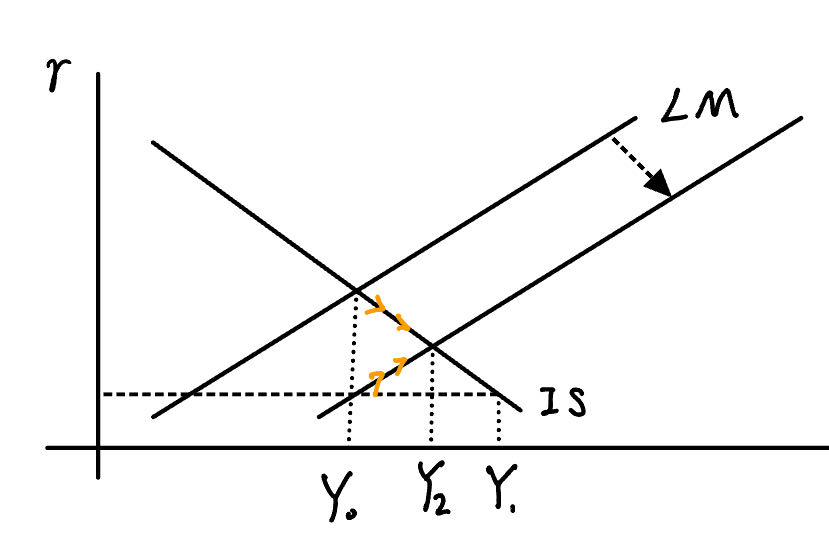
\includegraphics[width=\linewidth,height=0.9\textheight,keepaspectratio]{figures/fig23.png}

\caption{货币供给增加使 LM 曲线向下移动。产出从 $Y_0$ 升到 $Y_1$，利率从 $r_0$ 降到 $r_1$。}
\label{fig:macro-23}
\end{figure}

价格水平上升则让同一套机制反向运转。由于它压低了实际货币供给 $M/P$，它使 LM 曲线向上移动，抬高利率、压低产出。

\begin{figure}[h]
\centering
% original hand-drawn figure (kept as-is per author; TikZ parked in fig24_tikz.txt)
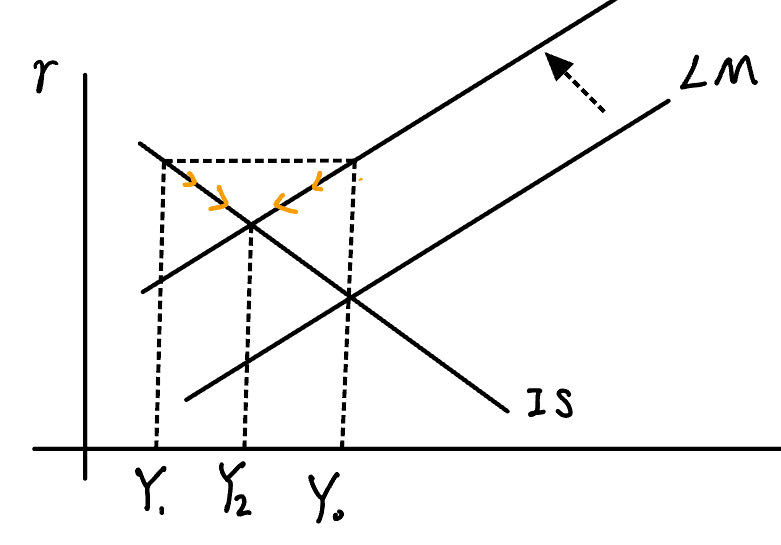
\includegraphics[width=\linewidth,height=0.9\textheight,keepaspectratio]{figures/fig24.png}

\caption{价格水平上升（实际货币供给 $M/P$ 下降）使 LM 曲线向上移动：利率升到 $r_1$，产出降到 $Y_1$。}
\label{fig:macro-24}
\end{figure}

最后这个实验值得停下来细想，因为它是 IS--LM 与下一章总需求曲线之间的关键枢纽：\emph{对货币市场而言，更高的价格水平等价于更小的货币供给}。于是，固定名义货币存量、只变动 $P$，就描出了价格水平与均衡产出之间的一种关系——而这恰恰就是总需求。

\state{小结}{
财政政策使 IS 曲线移动；货币政策（以及价格水平）使 LM 曲线移动。财政扩张抬高产出，但也抬高利率，从而挤出投资；货币扩张则通过压低利率来抬高产出。在每一种情形下，利率都会调整，使两个市场同时出清。
}
